%
% LaTeX template for ICAP 2010 abstracts.
%
\documentclass[10pt]{article}

\usepackage{graphicx}
\usepackage{icap2010}

\begin{document}
%%%%%%%%%   DO NOT MODIFY ANYTHING ABOVE THIS LINE %%%%%%%%

\title{Ultranarrow dark resonance in high temperature caesium cell using mode-locked Ti:sapphire laser and neon buffer gas}

\begin{authors}
  \author{G.}{Imreh}{1},
  \author{T-H.}{Wu}{1},
  \author{C-M.}{Wu}{1},
  \author{T-L.}{Yang}{1},
  \author{W-Y.}{Cheng}{1},
\end{authors}

\address{1}{Institute of Atomic and Molecular Sciences, Academia Sinica, Taiwan}

\begintext

Dark resonances due to coherent population trapping (CPT) offer naturally narrow line widths and are well suited for frequency standards. The width of these resonances can be reduced by using buffer gas. In continuous wave (CW) systems line width below 30Hz were previously observed in rubidium\footnote{M.~Erhard and H.~Helm, PRA {\bf 63}, 043813 (2001)}. To further improve this line width we use a mode-locked Ti:sapphire laser for optical pumping. This has the advantage that all interacting modes are in phase with each other, while in CW case the phase coherence of the pump lasers limits the achievable performance. Our system is unique in that the repetition rate and the offset frequency can be tuned independently \footnote{W-Y.~Cheng, T-H.~Wu, S-W.~Huang, S-Y.~Lin and C-M.~Wu, Applied Physics B {\bf 92}, 13 (2008)}. 

The repetition rate of the mode-locked laser is set to be near an integer multiple of the ground state hyperfine splitting of caesium (``clock frequency''), and by scanning the repetition rate we can probe the dark resonance. Compared to previous experiments\footnote{S.~Brattke, U.~Kallmann, and W.-D.~Hartmann,  Eur. Phys. J. D {\bf 3}, 159 (1998)} we use a different element and higher buffer gas temperature. In a cell buffered with 8700kPa neon at 100$^\circ$C we recorded 6.1(8)Hz line width (Figure 1). The expected large frequency shift of the resonance due to the buffer gas (several kHz) is absent, the observed shift is much smaller than the line width.

An optical clock based on such CPT signal using mode locked lasers will have the advantage of narrower resonance, much reduced systematic frequency shifting effects and because of its higher peak power the ability to use thicker optical medium thus achieving better signal-to-noise ratio.

We present our systematic studies of the this CPT signal and its theoretical analysis.

\begin{center}
  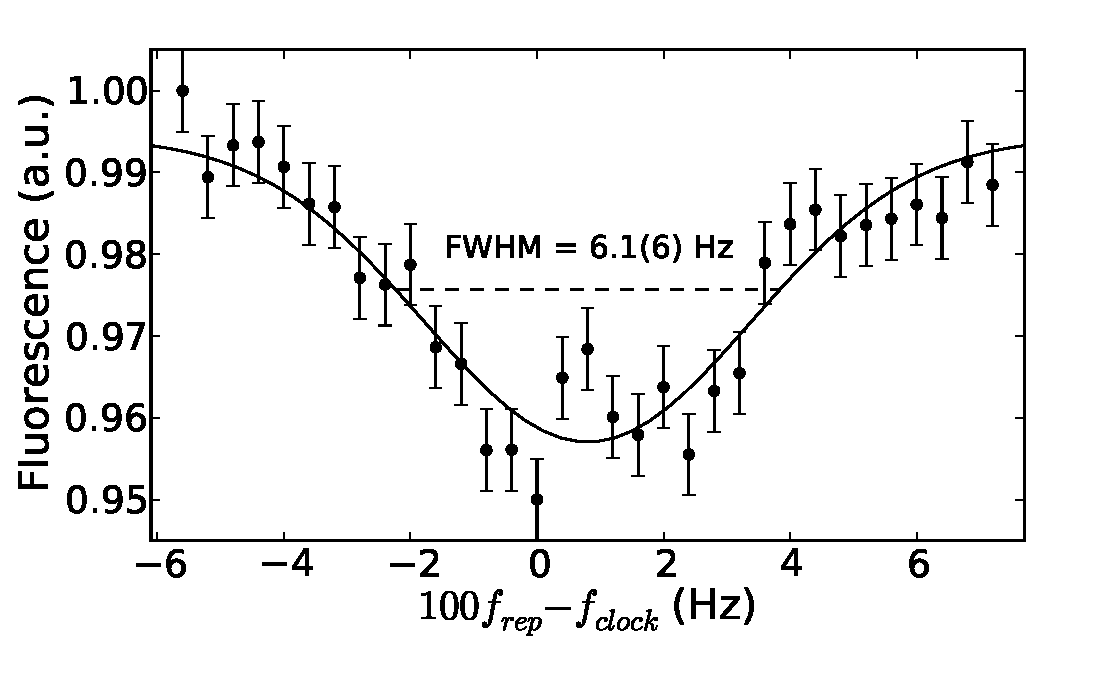
\includegraphics[width=0.5\textwidth]{8700Ne_buffer.eps}
\end{center}

\caption{1}{Dark resonance signal by tuning the mode locked laser's repetition rate}

%%%%%%%%%%   DO NOT MODIFY ANYTHING BELOW THIS LINE %%%%%%%%
\end{document}
